\documentclass[a4paper,9pt]{extarticle}
\usepackage[utf8]{inputenc}
\usepackage[T1]{fontenc}
\usepackage{graphicx}
\usepackage{xcolor}
\usepackage{tikz}

\usepackage{amsmath,amssymb,textcomp}
\everymath{\displaystyle}

\usepackage{times}
\renewcommand\familydefault{\sfdefault}
\usepackage{tgheros}
%\usepackage[defaultmono,scale=0.85]{droidmono}
\usepackage{multicol}
\setlength{\columnseprule}{0pt}
\setlength{\columnsep}{20.0pt}


\usepackage{geometry}
\geometry{
a4paper,
total={210mm,297mm},
left=10mm,right=10mm,top=10mm,bottom=15mm}

\linespread{1.3}


% custom title
\makeatletter
\renewcommand*{\maketitle}{%
\noindent
\begin{minipage}{0.4\textwidth}

\begin{tikzpicture}
\node[rectangle,rounded corners=6pt,inner sep=10pt,fill=blue!50!black,text width= 0.95\textwidth] {\color{white}\Huge \@title};
\end{tikzpicture}
\end{minipage}
\hfill
\begin{minipage}{0.55\textwidth}
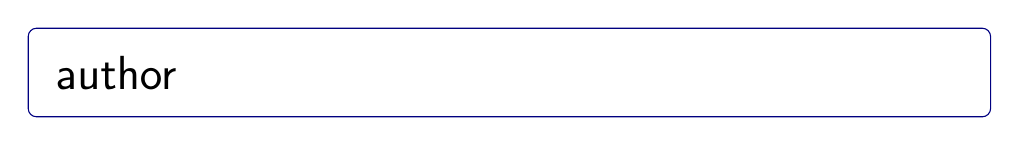
\begin{tikzpicture}
\node[rectangle,rounded corners=3pt,inner sep=10pt,draw=blue!50!black,text width= 0.95\textwidth] {\LARGE \@author};
\end{tikzpicture}
\end{minipage}
\bigskip\bigskip
}%
\makeatother




% custom footer
\usepackage{fancyhdr}
\makeatletter
\pagestyle{fancy}
\fancyhead{}
\fancyfoot[C]{\footnotesize \textcopyright\ \@date\ \ \@author}
\renewcommand{\headrulewidth}{0pt}
\renewcommand{\footrulewidth}{0pt}
\makeatother


\title{EE 212 - Equation Sheet\ Frequency Response}
\author{Victor Delaplaine}
\date{2018}



\begin{document}

\maketitle

\begin{multicols*}{3}


\section{Transfer Functions}


{Types of Transfer functions:}

$\tilde{H(\omega)} =  Voltage \; gain = \frac{\tilde{V_o}}{\tilde{V_i}}$ \\
$\tilde{H(\omega)} =  Current  \; gain = \frac{\tilde{I_o}}{\tilde{I_i}}$ \\
$\tilde{H(\omega)} =  Transfer \; Impedance = \frac{\tilde{V_o}}{\tilde{I_i}}$ \\
$\tilde{H(\omega)} =  Transfer \; admittance = \frac{\tilde{I_o}}{\tilde{V_i}}$ 


\subsection{Poles and Zeros

$\tilde{H(\omega)} = \frac{\tilde{N(\omega)}}{\tilde{D(\omega)}}$ \\
Where $\tilde{D(\tilde{p})} = 0 $ \\
$\tilde{N(\tilde{z})} = 0$ 

\section{Bels}
\includegraphics[width=0.4\columnwidth]{dBScale.png}

G = Number of bels = $log_{10}(\frac{P_o}{P_i})$ \\
$G_{dB} =  10 \cdot log_{10}(\frac{P_o}{P_i})$ \\
$G_{dB} = 20 \cdot log_{10}(\frac{I_o}{I_i}) $ \\
$G_{dB} = 20 \cdot log_{10}(\frac{V_o}{V_i}) $


\section{Resonant Circuits }

$\omega_1 = \omega_o [ \sqrt{1+ (\frac{1}{2Q})^2 }- \frac{1}{2Q}] $ \\
$\omega_2 = \omega_o [ \sqrt{1+(\frac{1}{2Q})^2 }+ \frac{1}{2Q}] $ \\

\subsection{RLC Series}

$\tilde{Z} = \tilde{H(s)} = R + j \omega L + \frac{1}{j \omega C} $ \\
 when $(\;  Im(\tilde{Z}(\omega_o)) = 0 \;\;)$ \\
 $\omega_o = \frac{1}{\sqrt{LC}}$
    
\subsubsection{ Series - Characteristics } 
$\omega_1 = - \frac{R}{2L} + \sqrt{({\frac{R}{2L}})^2 + \frac{1}{LC}}$ \\
$\omega_2 = \frac{R}{2L} + \sqrt{({\frac{R}{2L}})^2 + \frac{1}{LC}}$ \\
$\omega_o = \sqrt{\omega_1 \cdot \omega_2}$ \\
$B = \omega_2 - \omega_1$ \\
$Q = 2 \pi \frac{ maxium \; energy \; stored}{total \; energy \; lost \; per\; cycle\; at\; resonance} = 2\pi \frac{E_s}{E_D}$ \\


$E_s = \frac{1}{2}L i^2 + \frac{1}{2}C v_c^2$ \\
Assuming that: $v_c(t) =  V_C sin(\omega t)$ \\
$i = C \frac{dv_c}{dt} = \omega C V_c sin^2(\omega t)$ \\
$E_s(\omega_o) = \frac{1}{2}C V_c^2$ \\
$E_D(\omega_o) = (i(\omega_o)^2 * R) (\frac{1}{f_o}) $ \\
$Q = \frac{\omega_o L}{R} = \frac{1}{\omega_o RC}$ \\
$B = \frac{L}{R} = \frac{\omega_o}{Q}$ 

\subsection{RLC Parallel}

$\tilde{Z} = \tilde{H(s)} = R + j \omega L + \frac{1}{j \omega C} $ \\
when $(\;  Im(\tilde{Y}(\omega_o)) = 0 \;\;)$ \\
$\omega_o = \frac{1}{\sqrt{LC}}$ 
    

\subsubsection{Parallel - Characteristics } 

$\omega_1 = - \frac{1}{2RC} + \sqrt{({\frac{1}{2RC}})^2 + \frac{1}{LC}}$ \\
$\omega_2 = \frac{1}{2RC} + \sqrt{({\frac{1}{2RC}})^2 + \frac{1}{LC}}$ \\
$Q = \frac{\omega_o}{B} = \omega_o RC = \frac{R}{\omega_o L}$ \\
$B = \frac{1}{RC} $


\section{Passive Filters}
\includegraphics[width=0.4\columnwidth]{passiveFilterGraph.png}
   

\subsection{Low Pass Filter - RC}
\includegraphics[width=0.4\columnwidth]{LPF_RC.png} \\
$\tilde{H(\omega)} = \frac{\tilde{V_o}}{\tilde{V_i}} = \frac{1}{1+ j \omega * R * C} $ \\
$\omega_c = \frac{1}{RC}$

\subsection{High Pass Filter - RC}
\includegraphics[width=0.4\columnwidth]{HPF_RC.png} \\
$\tilde{H(\omega)} = \frac{\tilde{V_o}}{\tilde{V_i}} = \frac{j \omega R C}{1+ j \omega * R * C} $ \\
$\omega_c = \frac{1}{RC}$
 
\subsection{Band Pass Filter - RLC series} 
\includegraphics[width=0.4\columnwidth]{BPF_RLC.png} \\ 
$\tilde{H(\omega)} = \frac{\tilde{V_o}}{\tilde{V_i}} = \frac{ R }{R+ j (\omega L - \frac{1}{\omega C})} $ \\
$\omega_o = \frac{1}{\sqrt{LC}}$


\subsection{Band Stop Filter - RLC series}
\includegraphics[width=0.4\columnwidth]{BSF_RLC.png} \\
$\tilde{H(\omega)} = \frac{\tilde{V_o}}{\tilde{V_i}} = \frac{ j(\omega L - \frac{1}{\omega C}) }{R+ j (\omega L - \frac{1}{\omega C})}$ \\
$\omega_o = \frac{1}{\sqrt{LC}}$

\section{The End}

\end{multicols*}

\end{document}



